\section{Estimation of Model}

Only a single parameter of the model needs to be estimated: $\beta_L$. Again, just as when tuning the parameters driving the wage indirect inference is used. The parameters are tuned the following way. Simulate $N$ individuals. Find the relevant moments of supplied working hours. Find the mean squared distance between the actual supplied working hours and the simulated. Continue the process until convergence!

Usually when tuning a dynamic structural model, using simulated methods of moments one would supply the parameters not as part of the state space. The reason for this, is that as the size of the state space expands, it gets exponentially more expensive to solve the model. So the algorithm would go: for a given set of parameters need to be estimated, supply a random initialization. Solve the model for given parameters. Use the solved model to calculate the moments. Use numerical optimization to minimize given optimization problem.

\begin{figure}
    \centering
    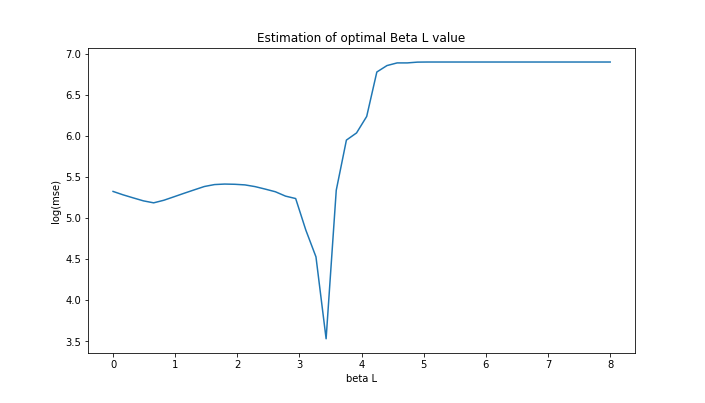
\includegraphics{figures/dqi_model1_estimation_Beta_L}
    \caption{Caption}
    \label{fig:dqi_model1_optimal_beta_L}
\end{figure}